\section{Reglerentwurf \buchSeite{80} \buch{232}}
\subsection{Stationärer Zustand und Fehler \buchSeite{80}}
\[ G_0(s) = K_0 \cdot \frac{1}{s^{\nu}} \cdot \underbrace{\text{"'Rest"'}}_\textrm{DC-Verstärkung = 1} \]
Die UTF des offenen Regelkreises setzt sich dabei aus derjenigen von Strecke
und Regler zusammen: $G_0(s) = G_S(s)\cdot G_R(s)$. Es wird davon ausgegangen, dass $G_0$
vollständig gekürzt ist und vom Typ $\nu$ ist d.h. $\nu$ offene Integratoren hat, bzw. $\nu$ Pole
bei Null:
\begin{table}[h!]
	\begin{tabularx}{\textwidth}{|l||X|X|X|}
        \hline
		& $r(t)=A\cdot\varepsilon(t) \quad $ Sprung & $r(t)=A\cdot t \quad$ Rampe & $r(t)=A\cdot \frac{t^2}{2} \quad$ Parabel \\ 
		\hline\hline
		$\nu =0 \ (Typ \ 0) \quad P-Verhalten$ & $e_\infty=\frac{A}{1+K_0}$ & $e_\infty=\infty$ & $e_\infty=\infty$ \\ \hline
		$\nu =1 \ (Typ \ 1) \quad  I-Verhalten$ & $e_\infty=0$ & $e_\infty=\frac{A}{K_0}$ & $e_\infty=\infty$ \\ \hline
		$\nu =2 \ (Typ \ 2) \quad  I^2-Verhalten$ & $e_\infty=0$ & $e_\infty=0$ & $e_\infty=\frac{A}{K_0}$ \\ \hline
	\end{tabularx}
\end{table}
\subsection{Spezifikationen für das dynamische Verhalten \buchSeite{83}}
\begin{equation*} 
	G_f(s)=\frac{Y(s)}{R(s)}=\frac{G_0(s)}{1+G_0(s)}
\end{equation*}
\begin{equation*}
	 \text{Sensitivität } S(s)=\frac{1}{1+G_0(s)} \qquad \text{komplementäre Sensitivität } T(s)=1-S(s)=\frac{G_0(s)}{1+G_0(s)}
\end{equation*}

\begin{center}
	\textbf{Ideal:} $\qquad S(s) = 0 \quad \rightarrow \quad T(s) =1 $
\end{center}

\begin{figure}[h]
	\begin{center}
	\begin{subfigure}[b]{8cm}
		\centering
		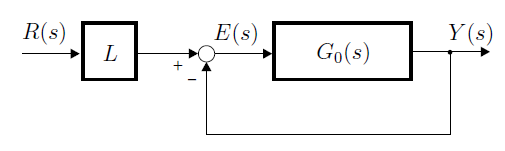
\includegraphics[width=7cm]{./images/regelkreismitL.png}
		\caption{Regelkreis mit Einheitsrückführung und Vorverstärkung L}
	\end{subfigure}\qquad
	\begin{subfigure}[b]{8cm}
		\centering
		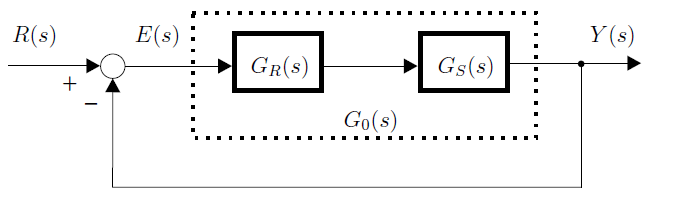
\includegraphics[width=7cm]{./images/RegelkreisEinheitsrueckfuehrung.png}
		\caption{Regelkreis mit Einheitsrückführung}
	\end{subfigure}
	\end{center}
\end{figure}
	Wird z.B. die Führungsgrösse mit einem Faktor bzw. Vorfilter L(s) vorverstärkt so ist $G_f(s)=\frac{Y(s)}{R(s)}=L(s)\cdot\frac{G_0(s)}{1+G_0(s)}$ während S(s) und T(s) erhalten bleiben.
%\begin{multicols}{2}
%		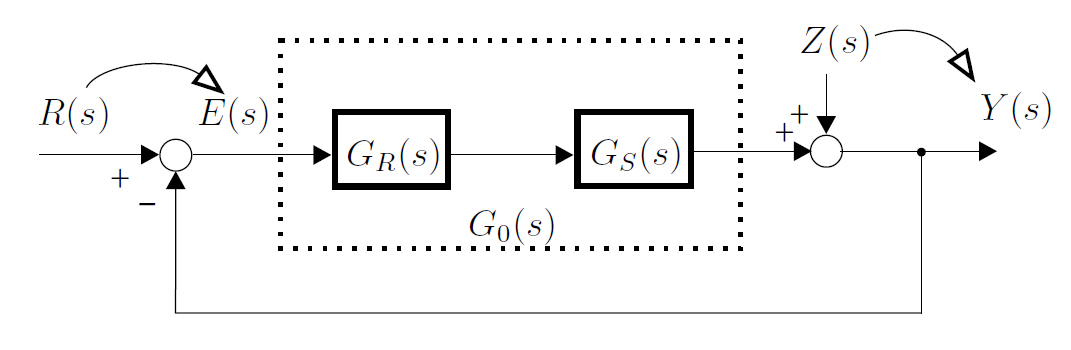
\includegraphics[width=9cm]{./images/SensitivitaetsUTF.png}
%\columnbreak
%
%Wegen $S(s) = \frac{1}{1+G_0(s)}$ ist auch der Verlauf von $S(j\omega)$ plausibel: kleine Verstärkung
%bei tiefen Frequenzen und $S(j\omega) \approx 1$ bei hohen Frequenzen. Abb. \ref{SensitivitaetRegelkreis} zeigt,
%dass $S(s) = \frac{E(s)}{R(s)}$ gilt; hochfrequente Führungssignale $r(t)$ erscheinen somit praktisch
%ungefiltert im Regelfehler $e(t)$. Ebenso wirken wegen $S(s) = \frac{Z(s)}{Y(s)}$ hochfrequente Störungen
%$z(t)$ am Streckenausgang fast ungefiltert auf die Regelgrösse $y(t)$.
%\end{multicols}

\begin{figure}[h!]
	\begin{center}
	\begin{subfigure}[b]{9cm}
	\flushleft
			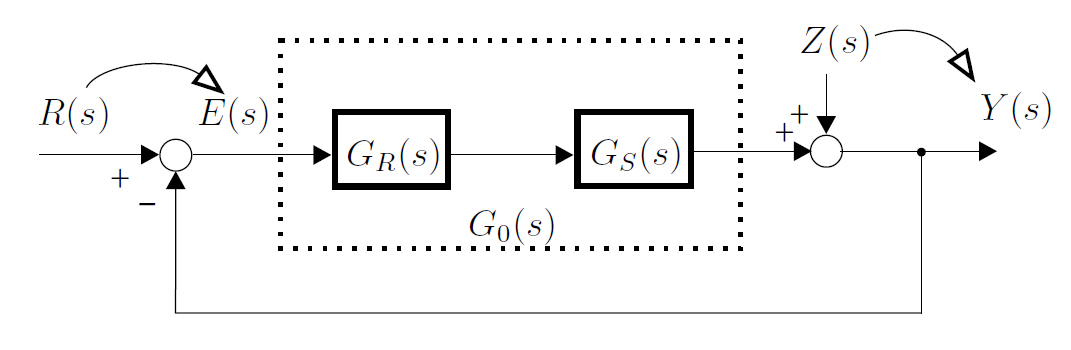
\includegraphics[width=9cm]{./images/SensitivitaetsUTF.png}
\caption{Sensitivitäts-UTF im Regelkreis, $S(s) = \frac{E(s)}{R(s)}=\frac{Z(s)}{Y(s)}$}
			\label{SensitivitaetRegelkreis}
	\end{subfigure}\qquad
	\begin{subfigure}[b]{8cm}
Wegen $S(s) = \frac{1}{1+G_0(s)}$ ist auch der Verlauf von $S(j\omega)$ plausibel: kleine Verstärkung
bei tiefen Frequenzen und $S(j\omega) \approx 1$ bei hohen Frequenzen. Abb. \ref{SensitivitaetRegelkreis} zeigt,
dass $S(s) = \frac{E(s)}{R(s)}$ gilt; hochfrequente Führungssignale $r(t)$ erscheinen somit praktisch
ungefiltert im Regelfehler $e(t)$. Ebenso wirken wegen $S(s) = \frac{Z(s)}{Y(s)}$ hochfrequente Störungen
$z(t)$ am Streckenausgang fast ungefiltert auf die Regelgrösse $y(t)$.

	\end{subfigure}
	\end{center}
\end{figure}



\subsection{Restriktionen: Bode-Integral der Sensitivität \buchSeite{87}}

Beim Erhöhen der Bandbreite $\omega_B$
besteht die Gefahr, dass in den Amplitudengängen von T und S Überhöhungen
entstehen. Werden T und S gemäss Abb. 63 als UTF T(s) = Y(s)/R(s) und
S(s) = E(s)/R(s) = Y (s)/Z(s) interpretiert, so ist auch klar, dass diese Überhöhungen
nachteilig sind. Oft wird deshalb die Spezifikationen ergänzt durch Maximalwerte für die Resonanzüberhöhung von
T und/oder S. Typische Maximalwerte sind z.B. 3-5 dB.

%\textbf{Theorem 3.1} (Bode-Integral der Sensitivität)\\
Es sei $G_0(s)$ eine gebrochen rationale Funktion mit mindestens zwei Polen mehr als Nullstellen, d.h. $n - m \geq 2$. $G_0(s)$ habe $N_p$ Pole $p_i$ in der rechten Halbebene. Dann gilt

\begin{equation}
\textrm{Bode-Integral der Sensitivität} \qquad
\int\limits_{0}^{\infty}ln|S(j\omega)|d\omega =\underbrace{\pi\cdot\sum\limits_{i=1}^{N_{p}}Re(p_i)}_\textrm{0, falls $G_0$ stabil}
\label{BodeIntegral}
\end{equation}

\begin{itemize}
	\item Ist $G_0$ stabil, dann wird der Ausdruck in (\ref{BodeIntegral}) gleich Null. Ist bei einer Frequenz
	$|S(j\omega)| < 0 \ dB$, dann muss zwingend irgendwo anders $|S(j\omega)| > 0 \ dB$ sein.
  \item Ist $G_0$ instabil, dann verschlechtert sich die Situation entsprechend.
	\item \textbf{Verkleinert man $|S(j\omega)|$ an einer Stelle, wird $|S(j\omega)|$ dafür an einer anderen
	Stelle grösser;} dies wird als ‘Wasserbetteffekt’ bezeichnet.
	Gleichung (\ref{BodeIntegral}) hat den Charakter eines Erhaltungsgesetzes.
	\item Bei den Frequenzen, bei denen
	der Aushub für ein bessere Bandbreite $\omega_B$ abgelagert wird, muss der Abstand zwischen dem Punkt -1 und der
	Ortskurve, d.h. $|1 + G_0|$, im Intervall $1 > |1 + G_0| \geq (1 + \varepsilon)-1$ liegen.
\end{itemize}

In der Praxis kann der Aushub also nicht einfach in einem beliebig hohen bzw.
breiten Frequenzband ‘entsorgt’ werden, sondern man muss Gleichung (\ref{BodeIntegral}) etwas
einschränken:
\begin{equation}
\int\limits_{0}^{\omega_M}ln|S(j\omega)|d\omega =\pi\cdot\sum\limits_{i=1}^{N_{p}}Re(p_i) \qquad \text{mit} \quad \omega_M \approx 10 \cdot \omega_B
\end{equation}